\documentclass[a4paper,11pt]{kth-mag}
\usepackage[T1]{fontenc}
\usepackage{textcomp}
\usepackage{lmodern}
\usepackage[latin1]{inputenc}
\usepackage[swedish,english]{babel}
\usepackage{modifications}
\usepackage{amsmath}
\usepackage{amsthm}
\usepackage{amssymb}
\usepackage{amsfonts}
\usepackage{hyperref}
\usepackage{graphicx}
\usepackage{enumitem}

\newcommand{\NN}{\ensuremath{\mathbb{N}}}
\newcommand{\ZZ}{\ensuremath{\mathbb{Z}}}
\newcommand{\QQ}{\ensuremath{\mathbb{Q}}}
\newcommand{\RR}{\ensuremath{\mathbb{R}}}
\newcommand{\CC}{\ensuremath{\mathbb{C}}}
\newcommand{\GG}{\ensuremath{\mathcal{G}}}

\newcommand{\Cpp}{\texttt{C++}}
\newcommand{\Gcc}{\texttt{gcc}}
\newcommand{\Gtkmm}{\texttt{gtkmm}}
\newcommand{\Gtk}{\texttt{GTK+}}

\title{SimpleGraphPlotter v1.6}

\subtitle{Programkonstruktion f\"{o}r F, DD1342\\ Laboration 4A}
\foreigntitle{}
\author{Jim Holmstr\"{o}m\\\href{mailto:jimho@kth.se}{jimho@kth.se}}
\date{\today}
\blurb{Teacher: Ann Bengtson}

\trita{}
\begin{document}
\frontmatter
\pagestyle{empty}
\removepagenumbers
\maketitle
\selectlanguage{english}
\tableofcontents*
\mainmatter
\pagestyle{newchap}

\chapter{Introduction}
In the following part firstly the problem will be explained and secondly 
the requirements for a basic plotter will be enlisted.
A plotter is a program that can plot functions from strings which defines the 
functions by ordinary math syntax. 
This project uses \Cpp~ programming language and the 
\Gtkmm\footnote{Documentation, binaries and source can be found at: 
\href{http://www.gtkmm.org}{www.gtkmm.org}} wrapper for the 
\Gtk\footnote{Documentation, binaries and source can be found at: 
\href{http://www.gtk.org}{www.gtk.org}} toolkit to generate the graphical user interface. 
It is compiled with the \texttt{GNU} \Gcc compiler.

\section{Requirements}
A few basic things is needed to have a functioning math plotter:
\begin{enumerate}
\item Define a function given ordinary math syntax.
\item Parse the inputed function and plot it accordingly.
\item Add/Remove functions from plotarea.
\item Plotarea should be scrollable both vertical and horizontal.
\item Range should be fixed to the unit-cube.
        \footnote{This restriction will be handled in section \ref{sec:scope}}
\item Display axis of the plot.
\item Parser must be properly tested.
\end{enumerate}

\section{Scope}
\label{sec:scope}
The amount of functionality that is possible to put in a system like this is
almost endless so a few delimitations has to be made in order to complete the project.
The currently biggest restriction to the plotter is the lack of 
ability to zoom or change the range from the unit-cube.
No support for parametric nor complex functions.
\footnote{
    Since no native support in \Cpp~ for complex numbers which means 
    all the basic math functions would have to be rewritten in order for this to work.
}

\section{Assistance}
Besides the reference manuals for \Gtkmm~ and \Cpp~ no external help for 
this project was received.

\chapter{Structure}
An basic overview of the structure can be seen in figure \ref{fig:UML}, all
public non-self-explanatory parts will then be enlisted and explained in 
a \verb+javadoc+ like manner. In the actual code the definition and
implementation was separated into \texttt{.h} and \texttt{.cpp}-files
respectively as long as possible,\footnote{Some small trivial methods where
left out from this distinction as well as a few things that is hard or
impossible to separate in \Cpp.} in a \Cpp~ manner and it mostly follows Google's
style guide for \Cpp.
\footnote{The style guide can be found at:
\href{
    http://google-styleguide.googlecode.com/svn/trunk/cppguide.xml
    }{
    google-styleguide.googlecode.com
    }
} 
The main goal of the structure for this project is to have as flexible code as possible.
\begin{figure}[ht]
\begin{center}
    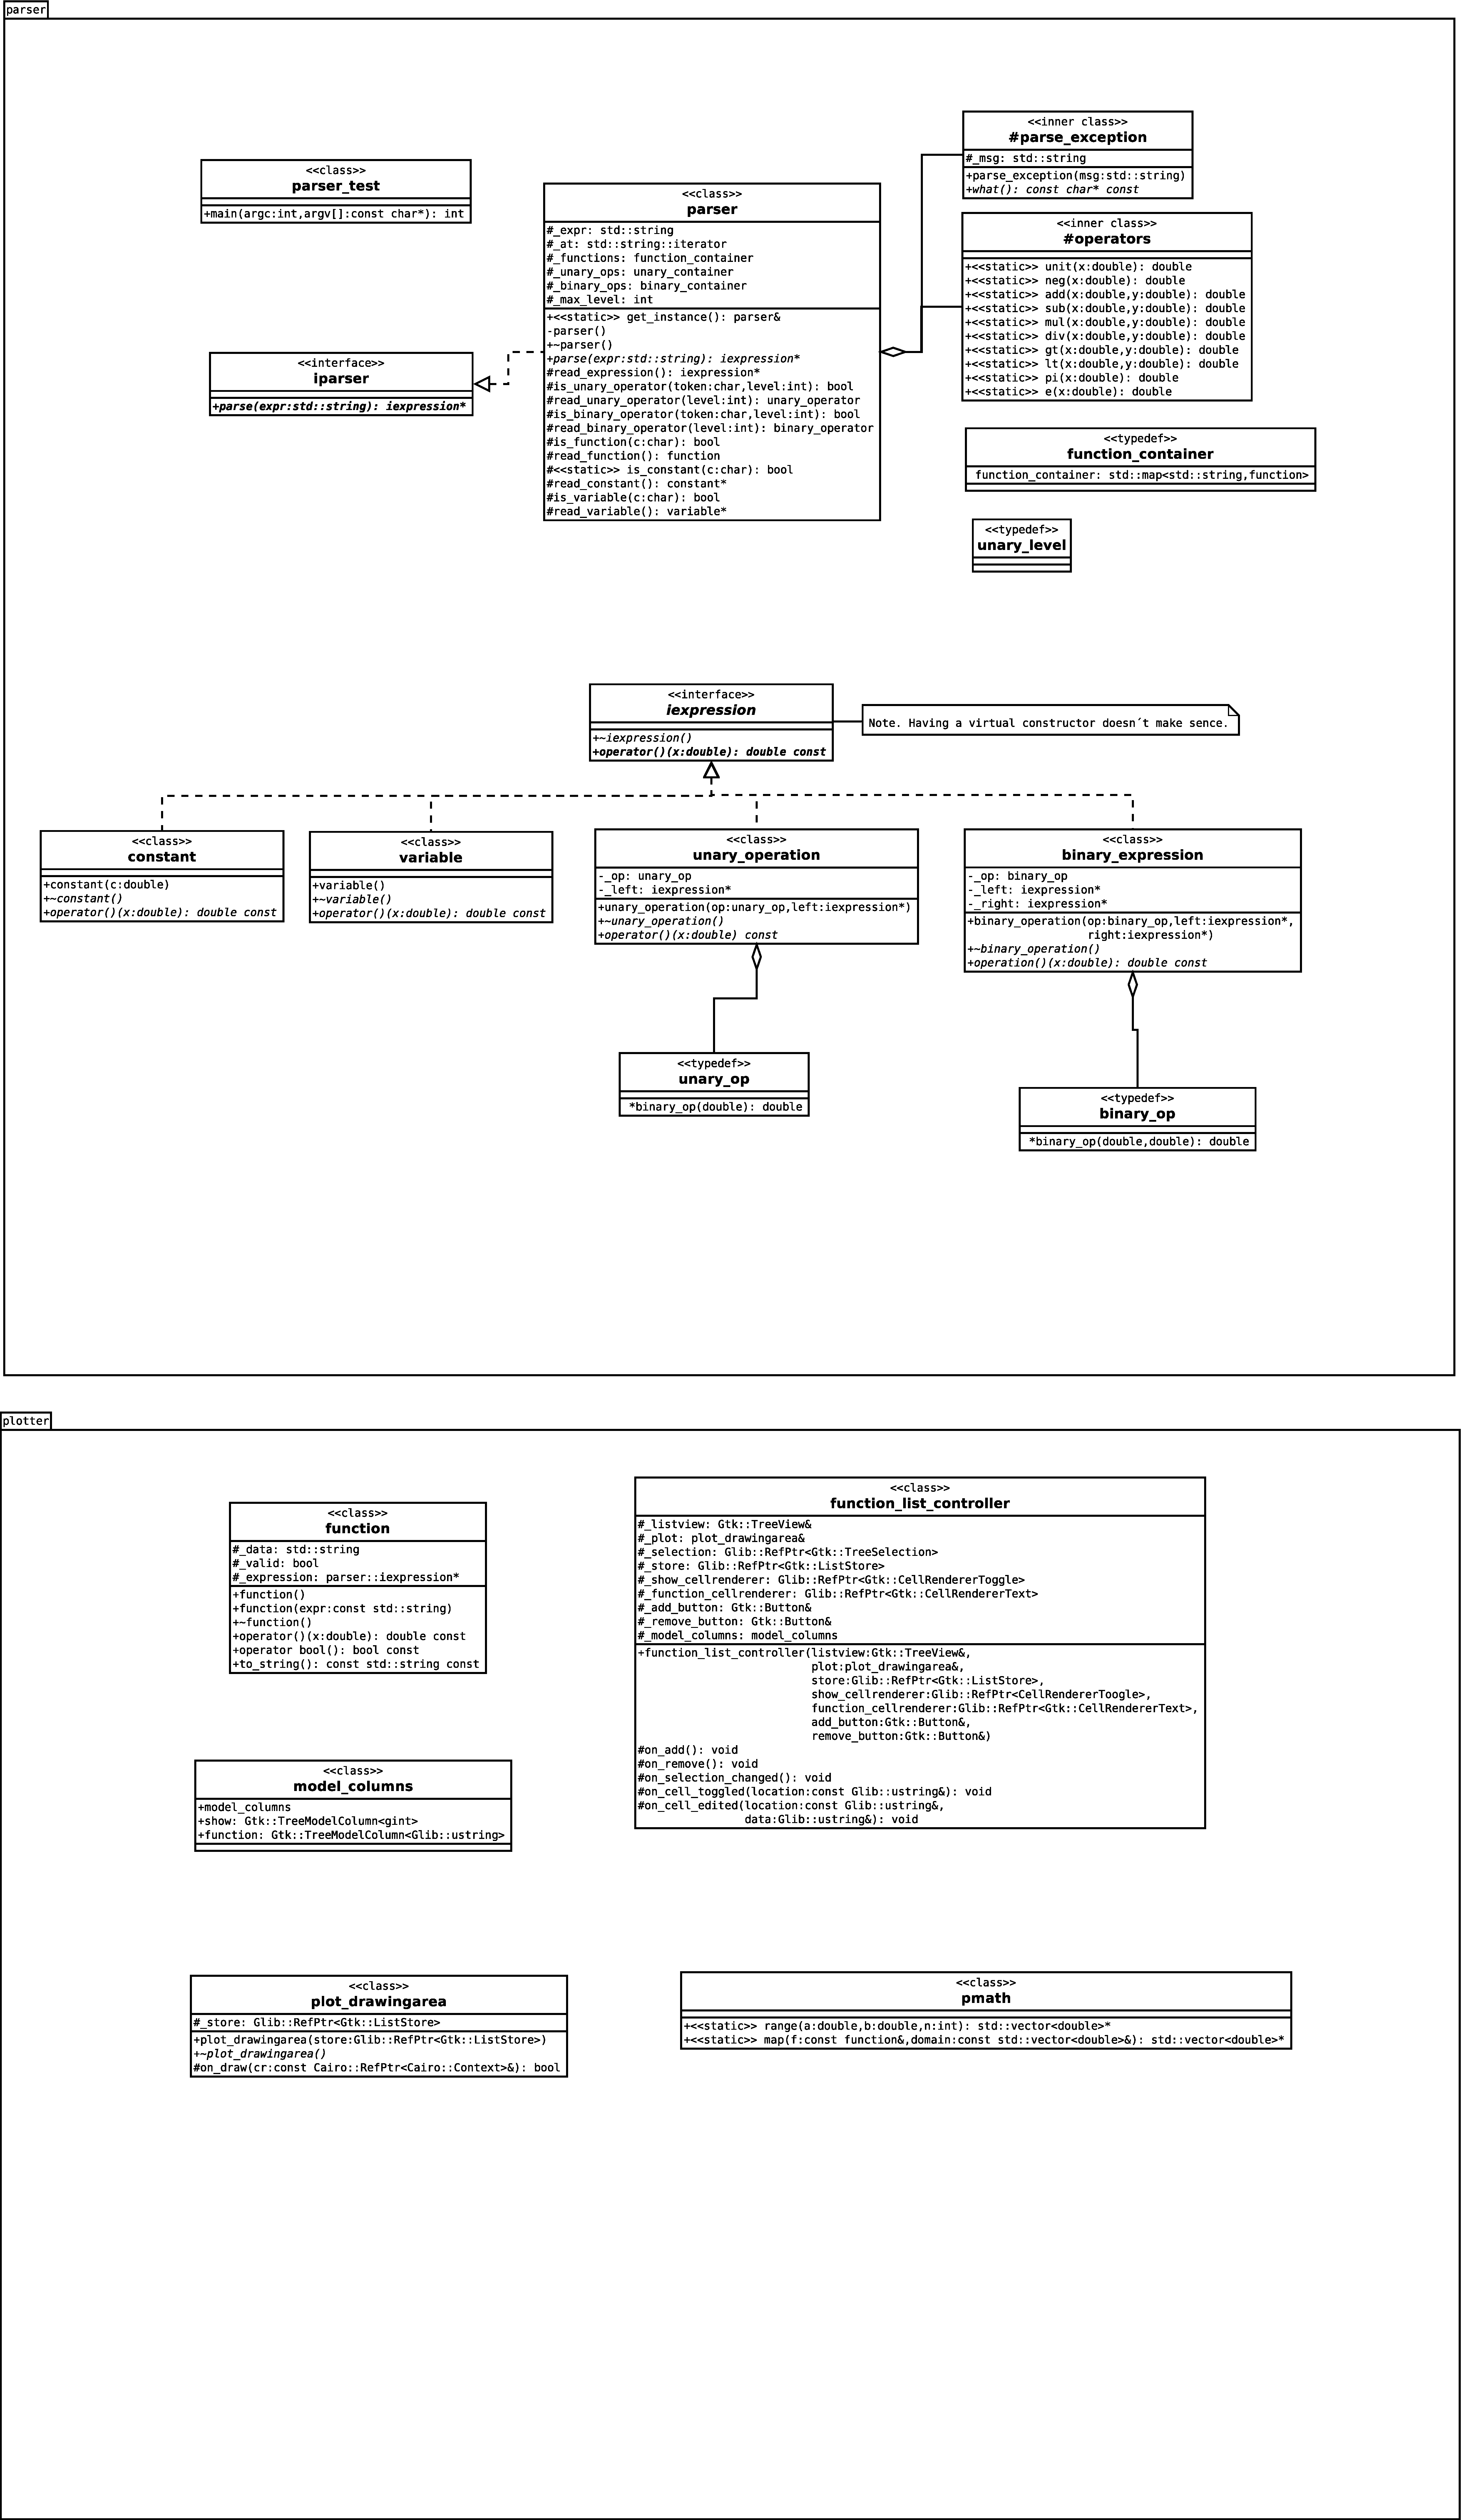
\includegraphics[width=0.75\textwidth]{uml.pdf}
    \caption{\small{An UML showing the structure and the enclosure.}}\label{fig:UML}
\end{center}
\end{figure}

\section{Parser}
The parser code can be divided into to parts the algorithm code, that is the 
actual parser, and the data structure in the form of a parse tree. 

\begin{figure}[ht]
\begin{center}
    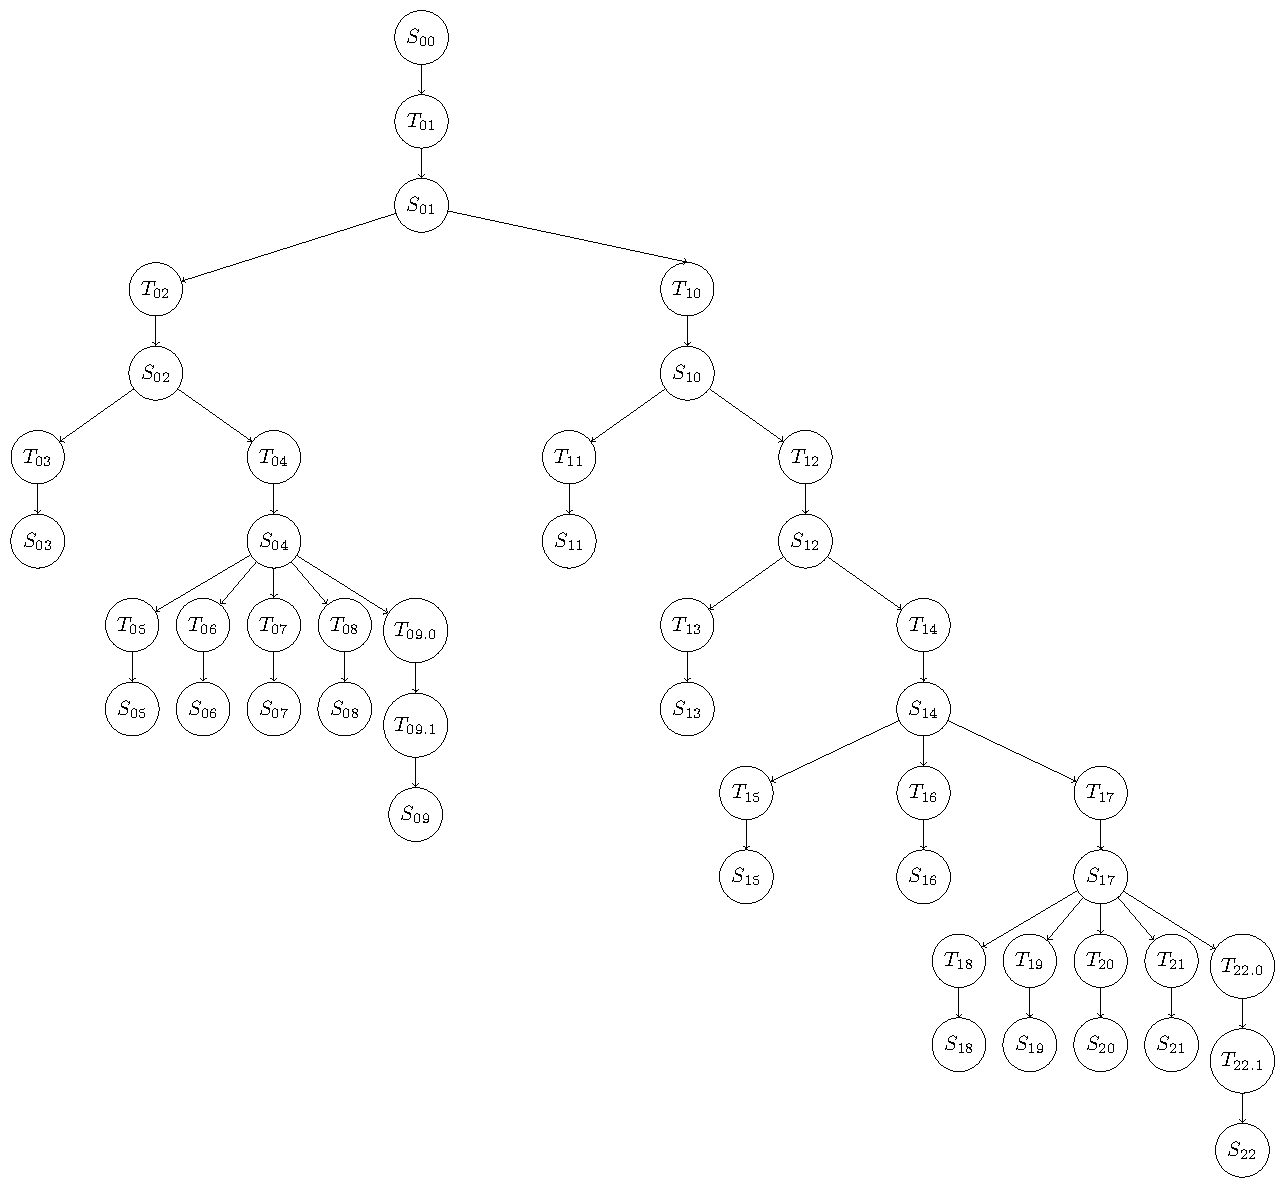
\includegraphics[width=0.5\textwidth]{parse-tree.pdf}
    \caption{\small{
        An example of the parse tree for the
        expression \texttt{sin(x+2)*(x-1)}\texttt{\^~}\!\!\texttt{5}.
        Trivial nodes from the generated by the actual implementation where
        here left out.
    }}
   \label{fig:parsetree}
\end{center}
\end{figure}

\subsection{interface iparser}
An \emph{abstract base class} (ABC) that defines the \emph{interface} for what a parser 
needs to have to be considered as a parser, in case for example
we want to compare different parser implementations.
\begin{description}
    \item[public parse(expr : std::string)] Virtual method that should be
    overloaded so that it will parse the string \texttt{expr} to
    generate a parse tree that represents the math expression in \texttt{expr}.
    \begin{description}
        \item[Parameters:]~\\
            \verb+expr+ - The string to be parsed.
        \item[Returns:]~\\
            A pointer to the root of the parse tree.
    \end{description}
\end{description}

\subsection{class parser}
The parser is an implementation of a \emph{recursive descent parser}. Two
types of methods are used in the parsing, \texttt{is-a}\footnote{Starts with
\texttt{is\_}} and \texttt{read-it}\footnote{Starts with \texttt{read\_}}.
The \texttt{is-a} is used for look-ahead to determine which type of expression
that lays ahead, while \texttt{read-it} is used to do the actual syntactic 
information gathering from the expression fragment.

>>>>>>>>TODO, note about the static things<<<<<<<<

The EBNF syntax for the parsing made by this algorithm is as follows:\\
\begin{verbatim}
    plots  = term-(-1),[';',expression-(-1)],'\n' (* no support for ';' this \\
    implementation *) (* -1 is the lowest order expression *)
    expression-i = [unary-i],expression-(i+1),[op-(i+1),expression-i]
    term-n = var | num | [function],(,term-(-1),) \\
    (* n is the number of the highest order operator *)

    op-0 = '>' | '<'
    op-1 = '+' | '-'
    op-2 = '*' | '/' | '%'
    op-3 = '^'
    unary-3 = '+' | '-' | '*' 
    num = ? all numbers ?
    var = 'x'
    function = cos | sin | tan | acos | asin | atan | cosh \\
    | sinh | tanh | exp | log | log10 | sqrt | ceil | abs \\
    | floor | pi | e (* where pi and e are constant
    functions *)
\end{verbatim}
In the definition of \texttt{expression-i} either \texttt{unary-(i+1)} or
\texttt{op-(i+1)} is choosen. Unary, since on the left, has higher priority.


\begin{description}
    \item[public parse(expr : std::string)] Parses the string \texttt{expr} to
    generate a parse tree that represents the math expression in \texttt{expr}.
    \begin{description}
        \item[Parameters:]~\\
            \verb+expr+ - The string to be parsed.
        \item[Returns:]~\\
            A pointer to the root of the parse tree.
    \end{description}
\end{description}

\subsection{interface iexpression}
\label{sec:iexpression}
Acts as abstract base class (ABC) for a node in the parse
tree, as in for example the nodes in figure \ref{fig:parsetree}. The
\texttt{iexpression} is a \emph{functor} since it has overloaded the
\texttt{operator} and can thus be called in the same way as any other function.
The \texttt{operator} can be both 
\emph{recursively} implemented, as in
    \texttt{unary}\footnote{As can be seen in equation \ref{eq:unarydefined}.} 
    and
    \texttt{binary}\footnote{As can be seen in equation \ref{eq:binarydefined}.}
, or
\emph{explicitly} implemented, as in 
    \texttt{constant}\footnote{As can be seen in equation \ref{eq:constantdefined}.} 
    and
    \texttt{variable}\footnote{As can be seen in equation \ref{eq:variabledefined}.}
.
The operator function is generally defined by:
\begin{eqnarray}
    \label{eq:expressiondefined}
    \texttt{expression}: \RR &\rightarrow& \RR \nonumber \\
    x &\mapsto& \texttt{operator(}x\texttt{)} .
\end{eqnarray}

\begin{description}
    \item[public operator(x : double) double const] 
    Virtual definition of the \emph{evaluation} function for expressions. 
    Since the operator is going to act as an mathematical function one must be certain
    that it behaves like one, that is it does not modifies the functor when
    called.\footnote{In contrast to a method where that behaviour is allowed.}
    Therefore the \texttt{const} keyword has been added to prevent this
    from accidentally happening in the \emph{realizations}.
    \begin{description}
        \item[Parameters:]~\\
            \verb+x+ - Input value for the expression. 
        \item[Returns:]~\\
            The output value of this expression given the parameter \texttt{x}.
    \end{description}
\end{description}

\subsection{class constant} An \emph{realization} of \texttt{iexpression}
\ref{sec:iexpression} which represents a constant. To keep constancy with the
iexpression this is implemented as a constant-function:
\begin{eqnarray}
    \label{eq:constantdefined}
    \texttt{constant}: \RR &\rightarrow& \RR \nonumber \\
    x &\mapsto& c .
\end{eqnarray}
\begin{description}
    \item[public constant(c : double)] Constructor 
    that constructs the function in the equation \ref{eq:constantdefined}. 
    \begin{description}
        \item[Parameters:]~\\
            \verb+c+ - The value of the constant in the expression.
    \end{description}
\end{description}
\begin{description}
    \item[public operator(x : double) double const] 
    Explicit realization of \texttt{iexpression.operator} returning a
    constant.
    \begin{description}
        \item[Parameters:]~\\
            \verb+x+ - Input value of the expression, does not matter only
            there for compatibility reasons. 
        \item[Returns:]~\\
            The output value of the expression.
    \end{description}
\end{description}

\subsection{class variable} An realization of \texttt{iexpression}
\ref{sec:iexpression} which represents a variable. A variable can simply be
seen as a unit-function:
\begin{eqnarray}
    \label{eq:variabledefined}
    \texttt{variable}: \RR &\rightarrow& \RR \nonumber \\
    x &\mapsto& x .
\end{eqnarray}
\begin{description}
    \item[public unary\_operation(op : unary\_op, left : iexpression*)] Constructor 
    that constructs the function in the equation \ref{eq:variabledefined}. 
    \begin{description}
        \item[parameters:]~\\
            \verb+op+ - the unary operation performed, which is an \texttt{unary\_op}\footnote{typedefined to
            be a function pointer: \texttt{*unary\_op(double):double}.} .\\
            \verb+left+ - the inner expression on which to perform the
            operation on.
    \end{description}
\end{description}
\begin{description}
    \item[public operator(x : double) double const] 
    Explicit realization of \texttt{iexpression.operator} returning the value
    of the input.
    \begin{description}
        \item[Parameters:]~\\
            \verb+x+ - Input value of the expression.
        \item[Returns:]~\\
            The output value of the expression.
    \end{description}
\end{description}


\subsection{class unary\_operation} An realization of \texttt{iexpression}
\ref{sec:iexpression} which represents a unary operation, a function
constructed with \texttt{op} \texttt{left}:
\begin{eqnarray}
    \label{eq:unarydefined}
    \texttt{unary}:\RR &\rightarrow& \RR \nonumber \\
    x &\mapsto& \texttt{op(left(}x\texttt{))}. 
\end{eqnarray}

\begin{description}
    \item[public unary\_operation(op : unary\_op, left : iexpression*)] Constructor 
    that constructs the function in the equation \ref{eq:unarydefined}. 
    \begin{description}
        \item[Parameters:]~\\
            \verb+op+ - The unary operation performed, which is an \texttt{unary\_op}\footnote{Typedefined to
            be a function pointer: \texttt{*unary\_op(double):double}.} .\\
            \verb+left+ - The inner expression on which to perform the
            operation on.
    \end{description}
\end{description}
\begin{description}
    \item[public operator(x : double) double const] 
    Recursive realization of \texttt{iexpression.operator} returning the
    returned value of \texttt{left} through \texttt{op}, as in equation
    \ref{eq:unarydefined}.
    \begin{description}
        \item[Parameters:]~\\
            \verb+x+ - Input value for the \texttt{left} expression.
        \item[Returns:]~\\
            The returned value from the equation \ref{eq:unarydefined}.
    \end{description}
\end{description}

\subsection{class binary\_operation} An realization of \texttt{iexpression}
\ref{sec:iexpression} which represents a binary operation, that is a function
constructed with \texttt{op} and \texttt{left/right}:
\begin{eqnarray}
    \label{eq:binarydefined}
    \texttt{binary}: \RR &\rightarrow& \RR \nonumber \\
    x &\mapsto& \texttt{op(left(}x\texttt{),right(}x\texttt{))}.
\end{eqnarray}
\begin{description}
    \item[public binary\_operation(op : binary\_op, left : iexpression*, right :
    iexpression*)] Constructor that constructs the function in the equation
    \ref{eq:binarydefined}. 
    \begin{description}
        \item[Parameters:]~\\
            \verb+op+ - The unary operation performed, which is an
            \texttt{binary\_op}\footnote{Typedefined to
            be a function pointer: \texttt{*binary\_op(double,double):double}.} .\\
            \verb+left+ - The left expression on which to perform the
            operation on. \\
            \verb+right+ - The right expression on which to perform the
            operation on.
    \end{description}
\end{description}
\begin{description}
    \item[public operator(x : double) double const] 
    Recursive realization of \texttt{iexpression.operator} returning the
    returned values of \texttt{left} and \texttt{right} through \texttt{op},
    as in equation \ref{eq:binarydefined}.
    \begin{description}
        \item[Parameters:]~\\
            \verb+x+ - Input value for the expression.
        \item[Returns:]~\\
            The returned value from the equation \ref{eq:binarydefined}.
    \end{description}
\end{description}

\section{Plotter}
\begin{figure}[ht]
\begin{center}
    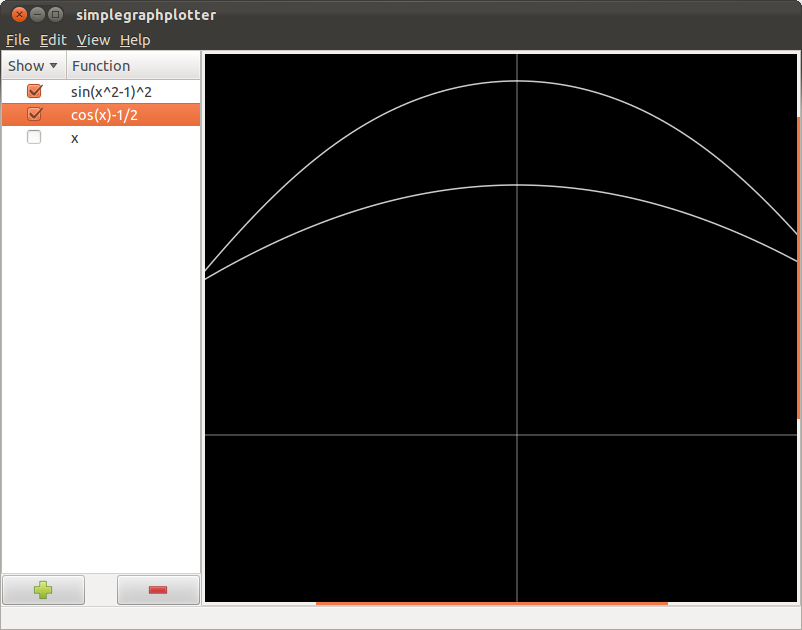
\includegraphics[width=0.75\textwidth]{screenshot00.png}
    \caption{\small{A screenshot of the program under normal operation.}}
   \label{fig:screenshot}
\end{center}
\end{figure}
\begin{figure}[ht]
\begin{center}
    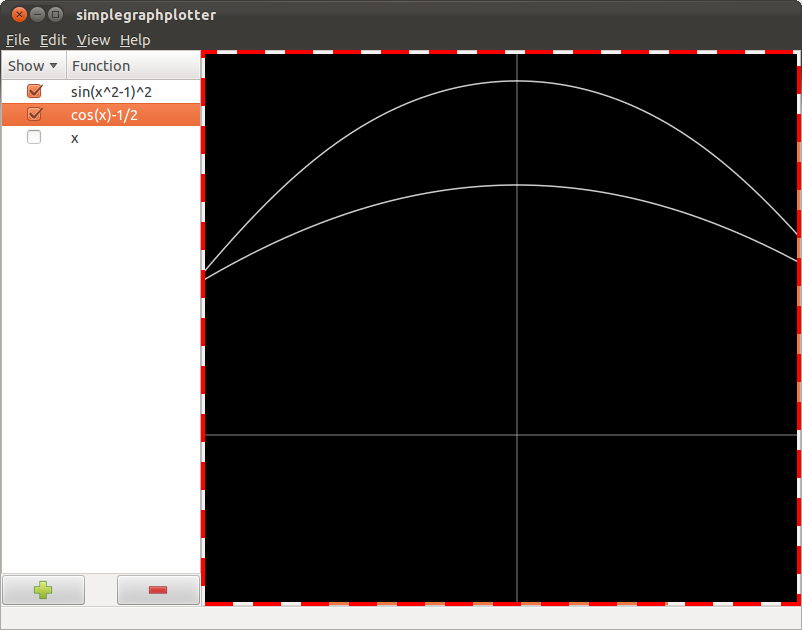
\includegraphics[width=0.75\textwidth]{screenshot00_plotarea.png}
    \caption{\small{A screenshot of the program under normal operation, with
    the plotarea highlighted.}}
   \label{fig:screenshotplotarea}
\end{center}
\end{figure}
\begin{figure}[ht]
\begin{center}
    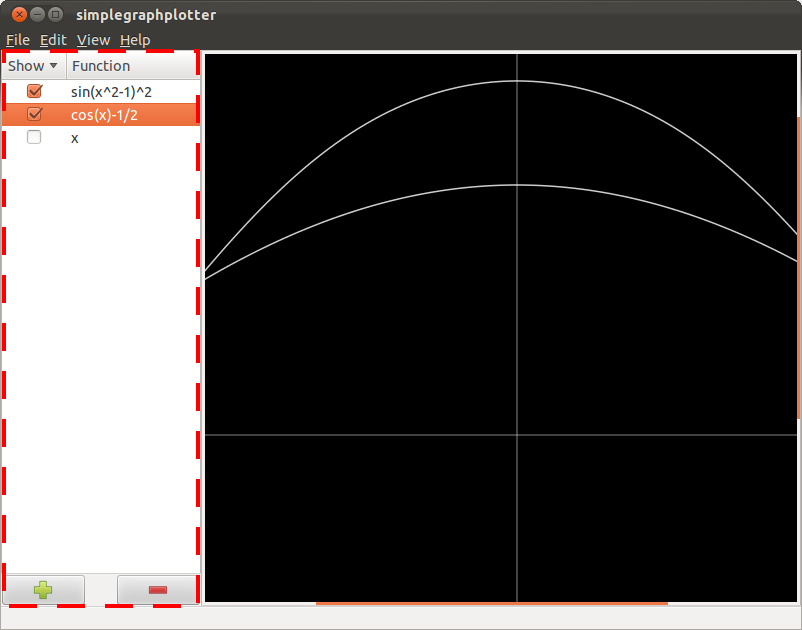
\includegraphics[width=0.75\textwidth]{screenshot00_function_list_controller.png}
    \caption{\small{A screenshot of the program under normal operation, with
    the view of the function\_list\_controller highlighted.}}
   \label{fig:screenshotfunctionlistcontroller}
\end{center}
\end{figure}


The GUI code for the plotter is separated 

MVC ?
V = plotdrawingarea
C = functionlistcontroller
M = what? (combined with something?)

>images with the different parts highlighted with a red border, that is the parts being described at the moment>
>especially point out the inheritance in the custom widgets.
>almost all layout is separetally defined in a .ui file\footnote{Follows XML
standard.} and loaded by the gtk \emph{builder} at startup.
>all signal connections are defined in main at generation. (main.cc)


\subsection{class function}
Acts as a model of a function which is used by \texttt{plot\_drawingarea}
TODO look how it is used, is it a model used by the view=plotdrawingarea...

It has the \emph{signature} for \texttt{iexpression} but it has not got the
same intended usage and should therefore not be a realization of
\texttt{iexpression}.

\begin{description}
    \item[public function(expr : const std::string)] Constructor 
    that constructs the function from the string \texttt{expr}.
    \begin{description}
        \item[parameters:]~\\
            \verb+expr+ - The expression to use as a function.
    \end{description}
\end{description}

\subsection{class plot\_drawingarea}

TODO
\begin{description}
    \item[public plot\_drawingarea(store : Glib::RefPtr<Gtk::ListStore>)] Constructor 
    that constructs \texttt{plot\_drawingarea}. 
    \begin{description}
        \item[parameters:]~\\
            \verb+store+ - Reference to the liststore that contains the
            functions to be rendered. Must be, or in the same format as
            \texttt{function\_store} defined in the \texttt{.ui}-file.
    \end{description}
\end{description}

\subsection{class function\_list\_controller}
TODO
\begin{description}
    \item[{
    \parbox[t]{\linewidth}
        {
        public function\_list\_controller(\\
            listview : Gtk::TreeView\&,\\
            plot : plot\_drawingarea\&,\\
            store : Glib::RefPtr<Gtk::ListStore>,\\ 
            show\_cellrenderer : Glib::RefPtr<Gtk::CellRendererText>,\\
            add\_button : Gtk::Button\&,\\
            remove\_button : Gtk::Button\&\\
            )
        }
    }]~\\
    Constructor that constructs... 
    \begin{description}
        \item[parameters:]~\\
            \verb+listview+ - \\
            \verb+plot+ - \\
            \verb+store+ - \\
            \verb+show_cellrenderer+ - \\
            \verb+add_button+ - \\
            \verb+remove_button+ - 
    \end{description}
\end{description}


\chapter{Results and Discussion}

\section{Results}
<<screenshots>>
Runned trough valgrind, results?.

\section{Discussion}
 = Problems with the unofficial \Cpp wrapper \Gtkmm, only used it to avoid
 missing out inheritance, polymorphism and to get it compatible with the
 standard \Cpp Library. Many normal things easily became hacky. 
 = Easy to miss combinations in the parser and have bugs.

\end{document}
